\documentclass[12pt, titlepage]{article}


\usepackage{array}
\usepackage{amssymb} 
\usepackage{float}
\usepackage{booktabs}
\usepackage{tabularx}
\usepackage{adjustbox}
\usepackage{longtable}
\usepackage{rotating}
\usepackage{hyperref}
\usepackage[round]{natbib}
\usepackage{caption}
\usepackage{graphicx}
\hypersetup{
    colorlinks,
    citecolor=black,
    filecolor=black,
    linkcolor=red,
    urlcolor=blue
}
\usepackage[round]{natbib}

\input{../Comments}
%% Common Parts

\newcommand{\progname}{Industrial Plant Designer} % PUT YOUR PROGRAM NAME HERE
\newcommand{\authname}{Team 18, Chemware Engineering
\\ Kishor Pandya
\\ Dhrumil Pandya
\\ Madhu Sivapragasam
\\ Rasik Pokharel} % AUTHOR NAMES                  

\usepackage{hyperref}
    \hypersetup{colorlinks=true, linkcolor=blue, citecolor=blue, filecolor=blue,
                urlcolor=blue, unicode=false}
    \urlstyle{same}
                                

\usepackage[normalem]{ulem} % for strikethrough
\graphicspath{ {./images/} }


\begin{document}

\title{Verification and Validation Report: \progname} 
\author{\authname}
\date{\today}
	
\maketitle

\pagenumbering{roman}

\section{Revision History}

\begin{tabularx}{\textwidth}{p{3cm}p{2cm}X}
\toprule {\bf Date} & {\bf Version} & {\bf Notes}\\
\midrule
March 3 & 1.0 & Madhu: Added some nfr tests and traceability matrix\\
March 4 & 1.0 & Madhu: Added module traceability matrix\\
March 5 & 1.1 & Kishor: Added some nfr tests and traceability matrix\\
March 5 & 1.2 & Kishor: Added answers in Appendix\\
March 6 & 1.3 & Dhrumil: Added some nfr tests and traceability matrix\\
March 6 & 1.4 & Rasik: Added fr tests \\
March 9 & 1.4 & Kishor: Added unit tests documentation\\
March 9 & 1.4 & Madhu: Added changes based off testing\\
March 10 & 1.4 & Rasik: Added nfr tests and tables and reflection\\
March 10 & 1.5 & Dhrumil: Added automated testing documentation\\
March 10 & 1.5 & Kishor: Added code coverage\\
\textcolor{blue}{April 2} & \textcolor{blue}{2.0} & \textcolor{blue}{Madhu: Updated failed tests and removed out of scope requirement}\\



\bottomrule
\end{tabularx}

~\newpage

\section{Symbols, Abbreviations and Acronyms}

\renewcommand{\arraystretch}{1.2}
\begin{tabular}{l l} 
  \toprule		
  \textbf{symbol} & \textbf{description}\\
  \midrule 
  T & Test\\
  \bottomrule
\end{tabular}\\


\newpage

\tableofcontents

\listoftables %if appropriate

\listoffigures %if appropriate

\newpage

\pagenumbering{arabic}

\section{Functional Requirements Evaluation}



\subsubsection{Tests for FR1}
\begin{enumerate}
\item{STN-FR1\\}

\textbf{Description:} The user must be able to create nodes in the product canvas.

\textbf{Type:} Functional, Dynamic, Manual

\textbf{Initial State:} The software is opened with a blank canvas thats setup with a new domain already selected.

\textbf{Input/Condition:} The user navigates to the sidebar and drags a new node onto the canvas.

\textbf{Output/Result:} The new node appears on the canvas with the correct icon and can be selected and moved easily.

\textbf{How the test will be performed:} A user will be asked to add a node to the blank canvas and then the output is verified by the user.

\textbf{Result:} Passed: The node appeared on the canvas with the correct icon and was movable.

\item{STN-FR2\\}

\textbf{Description:} The user must be able to update existing nodes on the product canvas.

\textbf{Type:} Functional, Dynamic, Manual

\textbf{Initial State:} The software is opened with a canvas that has a node already displayed in the canvas.

\textbf{Input/Condition:} The user selects a node and drags it to a new location.

\textbf{Output/Result:} The node moves to the new location.

\textbf{How the test will be performed:} A user will be asked to move a node from one location to another.

\textbf{Result:} Passed: The node was successfully moved to the new location.

\item{STN-FR3\\}

\textbf{Description:} The user must be able to delete a node from a canvas.

\textbf{Type:} Functional, Dynamic, Manual

\textbf{Initial State:} The software is opened with a canvas that has a node already displayed in the canvas.

\textbf{Input/Condition:} The user selects a node and presses backspace to delete it.

\textbf{Output/Result:} The node disappears from the canvas.

\textbf{How the test will be performed:} A user will be asked to delete a node from the canvas using backspace.

\textbf{Result:} Passed: The node was removed from the canvas after pressing backspace.

\end{enumerate}

\subsubsection{Tests for FR2}
\begin{enumerate}

\item{STN-FR4\\}

\textbf{Description:} The user must be able to select a node and input values for each of the node variables.

\textbf{Type:} Functional, Dynamic, Manual

\textbf{Initial State:} The software is opened with a blank canvas thats setup with a node appearing on the canvas.

\textbf{Input/Condition:} The user selects a node and adds values to each of the node variables.

\textbf{Output/Result:} The updated node now has values assigned to each variable which can be verified by selecting the node again.

\textbf{How the test will be performed:} A user will be asked to update the values for a specific node variable.

\textbf{Result:} Passed: The node variables were updated and verifiable upon reselection.

\item{STN-FR5\\}

\textbf{Description:} The user must be able to update stream values for the edge connection between two nodes.

\textbf{Type:} Functional, Dynamic, Manual

\textbf{Initial State:} The software is opened with a canvas that has a two nodes with an edge connecting them.

\textbf{Input/Condition:} The user selects the edge and updates the stream property.

\textbf{Output/Result:} The edge now has the selected stream property.

\textbf{How the test will be performed:} A user will be asked update the stream property of an edge connecting two nodes.

\textbf{Result:} Passed: The edge reflected the updated stream property.

\end{enumerate}

\subsubsection{Tests for FR3}
\begin{enumerate}
\item{STN-FR6\\}

\textbf{Description:} The user must be able to run a plant simulation model for a given plant design and then receive outputs based off of that simulation.

\textbf{Type:} Functional, Dynamic, Manual

\textbf{Initial State:} The software is opened with an existing plant model saved to the canvas.

\textbf{Input/Condition:} The user clicks the run button in order to run the simulation for that model.

\textbf{Output/Result:} The simulation is run and the outputs of the simulation are displayed to the user, the outputs should be equivalent to the outputs we get from using the excel solver model.

\textbf{How the test will be performed:} A user will be asked to run a simulation and then verify that the outputs match the outputs from the excel solver.

\textbf{Result:} Passed: The simulation ran and outputs matched the Excel solver results.

\end{enumerate}

\subsubsection{Tests for FR4}
\begin{enumerate}
\item{STN-FR7\\}

\textbf{Description:} The product must be able to display an error message if the user attempts to run a plant that is incomplete or has incorrect parameters.

\textbf{Type:} Functional, Dynamic, Manual

\textbf{Initial State:} The software is opened with an existing plant model with an unconnected pair of nodes.

\textbf{Input/Condition:} The user clicks the run button in order to run the simulation for that model.

\textbf{Output/Result:} An error message is displayed indicating that the pair of nodes is disconnected which means that the plant specified has an incorrect configuration.

\textbf{How the test will be performed:} A user will be asked to run a simulation for an incorrect plant model and then read an error message displayed from attempting to run that model.

\textbf{Result:} Passed: An error message correctly indicated the disconnected nodes.

\end{enumerate}

\subsubsection{Tests for FR5}
\begin{enumerate}
\item{STN-FR8\\}

\textbf{Description:} The product must be able to save existing canvas models into a local file format.

\textbf{Type:} Functional, Dynamic, Manual

\textbf{Initial State:} The software is opened with an existing plant model.

\textbf{Input/Condition:} The user clicks the save button in order to save the file locally.

\textbf{Output/Result:} The file should be saved locally to their local file system.

\textbf{How the test will be performed:} A user will be asked to save a model locally to their file system and then verify that the file exists in their local file system.

\textbf{Result:} Passed: The model was saved and verified in the local file system.

\end{enumerate}

\subsubsection{Tests for FR6}
\begin{enumerate}
\item{STN-FR9\\}

\textbf{Description:} The product must be able to restore files into the canvas from files stored in the local file storage.

\textbf{Type:} Functional, Dynamic, Manual

\textbf{Initial State:} The software is opened with a blank new plant canvas in the domain selection screen.

\textbf{Input/Condition:} The user clicks the restore button and then chooses to restore a file from their local filesystem.

\textbf{Output/Result:} The restored canvas should appear on the screen.

\textbf{How the test will be performed:} A user will be asked to restore a file from their local filesystem into the canvas and then check to make sure the model on the canvas matches what was on the local filesystem.

\textbf{Result:} Passed: The restored canvas matched the local file content.

\end{enumerate}

\subsubsection{Tests for FR7}
\begin{enumerate}
\item{STN-FR10\\}

\textbf{Description:} The user must be able to zoom into specific details on the canvas and observe the model closer.

\textbf{Type:} Functional, Dynamic, Manual

\textbf{Initial State:} The software is opened with a plant canvas with a detailed plant already existing on the canvas.

\textbf{Input/Condition:} The user double clicks to zoom into a certain section of the canvas.

\textbf{Output/Result:} The canvas will now be zoomed into that section of the model.

\textbf{How the test will be performed:} A user will be asked to zoom into a certain section of the plant canvas and then confirm that the product zooms into that section.

\textbf{Result:} Passed: The canvas zoomed into the specified section as expected.

\end{enumerate}

\subsubsection{Tests for FR8}
\begin{enumerate}

\item{STN-FR11\\}

\textbf{Description:} The user must be able to export the computation model output results into a csv file.

\textbf{Type:} Functional, Dynamic, Manual

\textbf{Initial State:} The software is opened with a plant canvas with a detailed plant already existing on the canvas and with the simulation run so that the output appears.

\textbf{Input/Condition:} The user clicks the export to csv button in order to export the data.

\textbf{Output/Result:} A csv is downloaded with all the output data stored to the csv.

\textbf{How the test will be performed:} A user will be asked to output the results of the computational model to a csv and then check the csv to confirm that the data matches what appears in the model outputs.

\textbf{Result:} Passed: The CSV file reflects the correct data

\end{enumerate}

\subsubsection{Tests for FR9}
\begin{enumerate}
\item{STN-FR12\\}

\textbf{Description:} The product must validate input data to make sure it is correct before the simulation runs.

\textbf{Type:} Functional, Dynamic, Manual

\textbf{Initial State:} The software is opened with a canvas that has a node displayed on it that has incorrect input data saved on to it such as a certain field without a corresponding value.

\textbf{Input/Condition:} The user clicks the run simulation button.

\textbf{Output/Result:} An error message is displayed indicating that one of the fields is missing a value.

\textbf{How the test will be performed:} A user will be asked to run the simulation for a node with incorrect input data and then read the error message thats returned when running the simulation to verify that errors are correctly provided.

\textbf{Result:} Passed: An error message correctly identified the missing field value.

\end{enumerate}

\subsubsection{Tests for FR10}
\begin{enumerate}
\item{STN-FR13\\}


\textbf{Description:} The product must provide realtime notifications for missing edges or nodes.

\textbf{Type:} Functional, Dynamic, Manual

\textbf{Initial State:} The software is opened with a canvas that has two nodes displayed that are missing a connection.

\textbf{Input/Condition:} The user does not connect the two nodes.

\textbf{Output/Result:} An indicator should appear that it makes it clear that an edge is missing.

\textbf{How the test will be performed:} A user will be asked to look at a canvas with two unconnected nodes and verify that an indicator appears that indicates there is a missing edge.

\textbf{Result:} Passed: An indicator appeared highlighting the missing edge.

\end{enumerate}



\section{Non-Functional Requirements Evaluation}

\subsubsection{Appearance Requirements}

\begin{enumerate}
    \item{STN-LAFAR1\\}

    \textbf{Description:} The product shall feature a clear and logically structured layout that organizes information hierarchically to reflect the plant’s structure and process flow.

    \textbf{Type:} Functional, Dynamic, Manual

    \textbf{Initial State:} The software is opened with a blank canvas.

    \textbf{Input/Condition:} The user navigates to select the domain for the plant model.

    \textbf{Output/Result:} The user interface will display the available models, which they can drag and drop onto the empty canvas. Users should be able to locate and navigate between different sections without confusion, and information must be presented clearly in a hierarchical manner.

    \textbf{How the test will be performed:} A group of users will be asked to complete specific tasks, such as finding a particular model and following the process flow. Feedback will be collected through a usability survey focused on layout clarity, evaluating aspects like ease of navigation and organization of information.

    \textbf{Result:} Passed: 9/10 users successfully completed the tasks of finding a specific model and tracing the process flow within 1 minute. The usability survey indicated an average rating of 4.5 out of 5 for layout clarity, with positive feedback highlighting intuitive navigation and well-organized information.

    \item{STN-LAFAR2\\}

\textbf{Description:} The product must use a consistent design across all elements, including fonts, colors, icons, and widgets, to ensure a cohesive and professional appearance.

\textbf{Type:} Functional, Dynamic, Manual

\textbf{Initial State:} The software is opened, displaying the main User Interface.

\textbf{Input/Condition:} The user is able to change the Canvas color between a light and dark theme.

\textbf{Output/Result:} The User Interface will reflect the selected theme (light or dark) across all elements. Specific color coding will apply to the models: input ports will be green, output ports will be red, and info ports will be blue.

\textbf{How the test will be performed:} Testers will evaluate the color scheme on multiple screens, ensuring adherence to the specified color guidelines and documenting any inconsistencies.

 \textbf{Result:} Passed: Testers confirmed that the color scheme adhered to the specified guidelines across five different screens (e.g., desktop, laptop, tablet), with consistent application of green for input ports, red for output ports, and blue for info ports. No inconsistencies were documented.

\item{STN-LAFAR3\\}

\textbf{Description:} The software must provide drag-and-drop functionality, allowing users to add, delete, rearrange, or modify elements such as reactor, source, separator, etc.

\textbf{Type:} Functional, Dynamic, Manual

\textbf{Initial State:} The software is opened, displaying the main User Interface with a blank Canvas.

\textbf{Input/Condition:} The user is able to drag and drop models onto the Canvas, rearrange them, and remove any dropped models as needed.

\textbf{Output/Result:} The User Interface will allow users to interact with models by dragging and dropping them onto the Canvas, with options to reposition or delete models. Changes made by the user are accurately reflected in the plant model hierarchy and layout.

\textbf{How the test will be performed:} A group of users will be asked to complete tasks involving the drag-and-drop functionality, such as adding specific models, rearranging them in a process flow, and deleting certain elements. Feedback will be collected via a usability survey focusing on ease of adding, arranging, and removing models, as well as the clarity of visual feedback for each action.
\textbf{Result:} Passed: 8/10 of users successfully completed the drag-and-drop tasks—adding three specific models, rearranging them into a process flow, and deleting two elements—within 2 minutes. The usability survey yielded an average score of 4.7 out of 5, with users praising the ease of adding, arranging, and removing models, and noting clear visual feedback (e.g., highlighted elements) for each action.

\end{enumerate}


\subsubsection{Style Requirements}
\begin{enumerate}
\item{STN-LAFSR1\\}

\textbf{Description:} The software must maintain sufficient contrast ratios between text, background colors, and interactive elements to ensure readability and accessibility.

\textbf{Type:} Functional, Dynamic, Manual

\textbf{Initial State:} The software is opened, displaying the main User Interface.

\textbf{Input/Condition:} The user navigates through various sections of the interface, including areas with text, background elements, and interactive components.

\textbf{Output/Result:} All text and interactive elements have a contrast ratio of at least 4.5:1 against their background colors, ensuring readability and accessibility compliance.

\textbf{How the test will be performed:} Using an accessibility tool or a color contrast analyzer, testers will measure contrast ratios for text and interactive elements against their backgrounds across different sections of the software. Any element with insufficient contrast will be documented for correction.

\textbf{Result:} Passed: Used a color contrast analyzer to measure contrast ratios across sections of the software ( canvas, sidebar, node modal), confirming that all text and interactive elements achieved a minimum contrast ratio of 4.5:1 against their backgrounds. No elements with insufficient contrast were documented.

\item{STN-LAFSR2\\}

\textbf{Description:} The software must utilize a neutral color scheme with professional accent colors reserved for emphasis and highlighting specific elements.

\textbf{Type:} Functional, Dynamic, Manual

\textbf{Initial State:} The software is opened, displaying the main User Interface with a default theme.

\textbf{Input/Condition:} The user navigates through various screens, observing the color scheme and accent colors used across the interface.

\textbf{Output/Result:} The interface displays a neutral base color palette with no more than three accent colors used only for actionable elements, alerts, or key information.

\textbf{How the test will be performed:} Testers will verify that the color scheme adheres to the neutral base and professional accent guidelines. Screenshots will be reviewed to confirm that accent colors are used consistently and only in areas requiring emphasis, and no more than three accent colors are visible at any time.

\textbf{Result:} Passed: Testers verified adherence to the neutral base and professional accent guidelines across ten screenshots from key UI sections (e.g., canvas, toolbar). Only three accent colors (blue, yellow, red) were consistently used for emphasis (e.g., buttons, alerts), with no deviations noted.

\item{STN-LAFSR3\\}

\textbf{Description:} The software must incorporate clear visual cues, such as highlighting, shading, or outlines, to indicate interactivity and selectable elements.

\textbf{Type:} Functional, Dynamic, Manual

\textbf{Initial State:} The software is opened, displaying various interactive components.

\textbf{Input/Condition:} The user interacts with elements such as buttons, models, and edges, observing visual feedback for each interaction.

\textbf{Output/Result:} Each interactive element visibly changes appearance (e.g., background color, border) when hovered over or selected, providing feedback on interactivity.

\textbf{How the test will be performed:} Testers will systematically hover over and select interactive elements, observing changes in visual cues such as color, shading, or outlines. Feedback consistency will be documented, and any interactive element that lacks appropriate visual feedback will be identified.

\textbf{Result:} Failed: Testers hovered over and selected 25 interactive elements (e.g., buttons, nodes, edges) across the UI, observing consistent visual cues—color changes (e.g., blue to light blue), shading, or outlines—for each. Some elements lacking feedback were identified (eg. Edges.) 

\textcolor{blue}{\textbf{Rev 1 Result:} Passed: After this test failed in revision 1, we added interactivity to all components that were missing visual cues and then reran the test with a different third party to ensure that it passed correctly. This time all interactive elements were observed to have visual cues successfully.}

\end{enumerate}


\subsubsection{Ease of Use Requirements}
\begin{enumerate}
\item{STN-UHE1\\}

\textbf{Description:} Each component of the service should be labeled with a descriptive tag that indicates what that component is used for.

\textbf{Type:} Functional, Dynamic, Manual

\textbf{Initial State:} The software is opened, displaying the main User Interface with all components accessible.

\textbf{Input/Condition:} The user examines each UI component to locate and read its associated label.

\textbf{Output/Result:} Each component has a unique, clear label that accurately describes its function, with no components left unlabeled or ambiguously labeled.

\textbf{How the test will be performed:} Testers will go through each UI component and confirm the presence of a descriptive label for each one. They will record any component that is missing a label or has an unclear or misleading label, ensuring that every component has a one-to-one relationship with its label.

\textbf{Result:} Failed: Testers reviewed 25 UI components (e.g., buttons, input fields, icons) and confirmed each had a unique, descriptive label (e.g., "Add Node," "Flow Rate"). Many missing, unclear, or misleading labels were recorded, violating a one-to-one label relationship.

\textcolor{blue}{\textbf{Rev 1 Result:} Passed: After this test failed in revision 1, we added labels to all components that were marked as missing labels and then reran the test with a different third party to ensure that it passed correctly. This time all were considered to be labeled successfully.}
\item{STN-UHE2\\}

\textbf{Description:} The UI control animations, such as dragging and dropping nodes and edges, should be smooth and without lag.

\textbf{Type:} Functional, Dynamic, Manual

\textbf{Initial State:} The software is opened with nodes and edges available for dragging and dropping onto the canvas.

\textbf{Input/Condition:} The user performs drag-and-drop actions with nodes and edges, observing the smoothness of the animation.

\textbf{Output/Result:} All animations run smoothly without buffering or lag, allowing users to seamlessly move nodes and edges on the canvas.

\textbf{How the test will be performed:} Testers will interact with the drag-and-drop elements, observing animation smoothness and responsiveness. Feedback will be gathered from testers and optionally from third-party reviewers, who will rate the smoothness of the animations. Any instances of lag or buffering will be noted for refinement.

\textbf{Result:} Passed: Testers dragged and dropped 15 elements (e.g., nodes, edges), noting smooth animations with no lag or buffering. Feedback from five testers and three third-party reviewers averaged a 4.8/5 smoothness rating, with no refinement needs identified.
\end{enumerate}

\subsubsection{Personalization and Internationalization Requirements}

\begin{enumerate}

\item{STN-UHPI-1\\}

\textbf{Description:} The system will use English everywhere throughout the system.

\textbf{Type:} Functional, Dynamic, Manual

\textbf{Initial State:} The software is opened, displaying the main interface and all accessible screens and components.

\textbf{Input/Condition:} The tester navigates through all screens, features, and tooltips within the system, observing any text elements (e.g., labels, buttons, notifications).

\textbf{Output/Result:} All text within the system is displayed in English, with no text appearing in other languages or being left untranslated.

\textbf{How the test will be performed:} Testers will systematically go through each part of the user interface, checking that all text elements, including error messages, tooltips, menus, and labels, are written in English. Any occurrences of non-English text or untranslated phrases will be documented for correction.

\textbf{Result:} Passed: Testers examined 50 text elements (e.g., error messages like "Invalid Input," tooltips, menu options) across all UI parts, confirming all were in English. No non-English text or untranslated phrases were documented.

\end{enumerate}

\subsubsection{Learning Requirements}

\begin{enumerate}

\item{STN-UHL-1\\}

\textbf{Description:} There should be documentation that enables a new user to learn the system.

\textbf{Type:} Functional, Dynamic, Manual

\textbf{Initial State:} The software is opened, displaying the main interface and access to documentation through the support tab.

\textbf{Input/Condition:} The user accesses the documentation while using the system for the first time.

\textbf{Output/Result:} New users are able to understand and follow the documentation to perform basic tasks within the system.

\textbf{How the test will be performed:} New users will be asked to complete a set of predefined tasks using the documentation. Observations will be made on whether users can successfully learn the system and complete tasks within half an hour.

\textbf{Result:} Passed: Ten new users completed five predefined tasks (e.g., adding a node, running a simulation) using the documentation within an average of 25 minutes. All users successfully learned the system, with no failures observed.

\item{STN-UHL-2\\}

\textbf{Description:} The system controls should be intuitive and easy to understand such that a new user can easily understand how to operate it.

\textbf{Type:} Functional, Dynamic, Manual

\textbf{Initial State:} The software is opened, displaying the main user interface.

\textbf{Input/Condition:} New users interact with the controls of the system for the first time.

\textbf{Output/Result:} New users should be able to see a tutorial which will help them to operate the system without confusion, with no more than one question regarding how to use the controls.

\textbf{How the test will be performed:} A group of new users will be observed as they navigate and use the system. Any questions or difficulties encountered during their interaction will be documented and analyzed.

\textbf{Result:} Passed: Eight new users navigated the system, completing basic operations (e.g., model creation, editing) in 2 minutes. Only one user asked a single question ("How to save?"), with no significant difficulties documented, indicating intuitive use.

\end{enumerate}

\subsubsection{Speed and Latency Requirements}

\begin{enumerate}

\item{STN-PS1\\}

\textbf{Description:} User inputs/interactions into the system should have a less than 60 ms latency.

\textbf{Type:} Performance, Dynamic, Automated

\textbf{Initial State:} The software is running and ready for user interaction.

\textbf{Input/Condition:} User performs actions such as adding, moving, or deleting nodes/edges on the canvas.

\textbf{Output/Result:} The system should process user inputs with a latency of less than 60 ms.

\textbf{How the test will be performed:} Automated scripts will measure the time from the moment an input is registered until the corresponding GUI output is displayed, ensuring it is less than 60 ms.

\textbf{Result:} Passed: The latency was consistently below 60 ms.

\item{STN-PS2\\}

\textbf{Description:} Saving a schema to a filesystem should take less than 1 second.

\textbf{Type:} Performance, Dynamic, Automated

\textbf{Initial State:} The software is running with a schema ready to be saved.

\textbf{Input/Condition:} User initiates the save operation for a schema.

\textbf{Output/Result:} The schema should be saved to the filesystem within 1 second.

\textbf{How the test will be performed:} Automated tests will track the time taken from the initiation of the save operation to its completion, ensuring it is less than 1 second.

\textbf{Result:} Passed: The save operation completed within 1 second.

\item{STN-PS3\\}

\textbf{Description:} Restoring a schema from the filesystem should take less than 1 second.

\textbf{Type:} Performance, Dynamic, Automated

\textbf{Initial State:} The software is running and a previously saved schema is available.

\textbf{Input/Condition:} User initiates the restore operation for a schema.

\textbf{Output/Result:} The schema should be restored from the filesystem within 1 second.

\textbf{How the test will be performed:} Automated tests will measure the time taken to complete the restore operation, ensuring it is less than 1 second.

\textbf{Result:} Passed: The restore operation completed within 1 second.

\item{STN-PS4\\}

\textbf{Description:} Running the factory simulation model and getting outputs should take no longer than 10 seconds.

\textbf{Type:} Performance, Dynamic, Automated

\textbf{Initial State:} The software is running, and the simulation model is prepared for execution.

\textbf{Input/Condition:} User initiates the simulation run for the factory model.

\textbf{Output/Result:} The output from the simulation should be returned within 10 seconds.

\textbf{How the test will be performed:} Automated scripts will measure the time taken from the start of the simulation until the output is generated, ensuring it is within the 10-second limit.

\textbf{Result:} Passed: The simulation completed within 10 seconds.

\end{enumerate}

\subsubsection{Precision or Accuracy Requirements}

\begin{enumerate}

\item{STN-PPA1\\}

\textbf{Description:} All numerical user inputs will not be constrained or rounded by the system.

\textbf{Type:} Functional, Dynamic, Manual

\textbf{Initial State:} The software is open, allowing user input for numerical values.

\textbf{Input/Condition:} User enters numerical values without any constraints.

\textbf{Output/Result:} The system should accept and process all numerical inputs as entered.

\textbf{How the test will be performed:} Testers will input various numerical values into the system and verify that no rounding or constraints are applied, ensuring that all inputs are passed directly to the external processing model.

\textbf{Result:} Passed: All numerical inputs were accepted without rounding or constraints.

\item{STN-PPA2\\}

\textbf{Description:} All graphical user inputs (creating/editing/deleting nodes and edges) that are shown via the GUI will be sent to the model as what’s shown on the canvas.

\textbf{Type:} Functional, Dynamic, Manual

\textbf{Initial State:} The software is open, and a canvas is being edited.

\textbf{Input/Condition:} User creates, edits, or deletes nodes and edges on the canvas.

\textbf{Output/Result:} The data sent to the processing model should match the graphical representation shown on the canvas.

\textbf{How the test will be performed:} Testers will manipulate the canvas and then check the data sent to the external model to ensure it matches exactly with what is displayed on the canvas.

\textbf{Result:} Passed: All graphical inputs were correctly reflected in the data sent to the model.

\end{enumerate}

\subsubsection{Robustness or Fault-Tolerance Requirements}

\begin{enumerate}

\item{STN-PRF1\\}

\textbf{Description:} All failures or errors that the model produces will be displayed to the user with information regarding the error or failure.

\textbf{Type:} Functional, Dynamic, Manual

\textbf{Initial State:} The software is running, and the external processing model is operational.

\textbf{Input/Condition:} An operation is performed that triggers an error in the external processing model.

\textbf{Output/Result:} The user should see a context box displaying information about the error/failure.

\textbf{How the test will be performed:} Testers will deliberately cause errors in the external model and verify that appropriate error messages are displayed to the user, including detailed information regarding the issue.

\textbf{Result:} Passed: Error messages were displayed correctly with detailed information.

\item{STN-PRF2\\}

\textbf{Description:} All failures and errors from the system should be shown to the user with information regarding the error/failure.

\textbf{Type:} Functional, Dynamic, Manual

\textbf{Initial State:} The software is running, and a user is interacting with the system.

\textbf{Input/Condition:} An error occurs within the system (not related to the external model).

\textbf{Output/Result:} The user should see a context box with information about the error/failure.

\textbf{How the test will be performed:} Testers will trigger various scenarios that result in system errors and check that the corresponding error messages are displayed to the user with clear, helpful information.

\textbf{Result:} Passed: System errors were displayed with clear, helpful information.

\end{enumerate}

\subsubsection{Capacity Requirements}

\begin{enumerate}

\item{STN-PC1\\}

\textbf{Description:} The system should be able to handle schemas with up to 100 nodes and 1000 edges.

\textbf{Type:} Functional, Dynamic, Manual

\textbf{Initial State:} The software is open and ready for schema creation.

\textbf{Input/Condition:} User creates a schema with up to 100 nodes and 1000 edges.

\textbf{Output/Result:} The system should successfully handle the schema without performance degradation.

\textbf{How the test will be performed:} Testers will create schemas that include 100 nodes and 1000 edges, monitoring the system’s performance and responsiveness during and after the creation process.

\textbf{Result:} Passed: The system handled the schema with 100 nodes and 1000 edges without performance issues.

\end{enumerate}

\subsubsection{Scalability or Extensibility Requirements}

\begin{enumerate}

\item{STN-PSE1\\}

\textbf{Description:} The system should only need to be scalable to handle a single user.

\textbf{Type:} Performance, Dynamic, Automated

\textbf{Initial State:} The software is running, simulating a single user environment.

\textbf{Input/Condition:} Simulated user inputs are made to test the system’s performance.

\textbf{Output/Result:} The system should handle all user inputs without performance issues.

\textbf{How the test will be performed:} Automated scripts will simulate user inputs and interactions with the system, testing its performance under load to ensure it can handle all inputs efficiently from a single user.

\textbf{Result:} Passed: The system efficiently handled all inputs from a single user.

\end{enumerate}

\subsubsection{Longevity Requirements}

\begin{enumerate}

\item{STN-PL1\\}

\textbf{Description:} The system should be maintainable without developer interference for at least 1 year.

\textbf{Type:} Maintenance, Dynamic, Manual

\textbf{Initial State:} The system is operational and ready for handover to the sponsor.

\textbf{Input/Condition:} The system is used without developer support for a year.

\textbf{Output/Result:} The system remains operational and usable after one year without significant issues.

\textbf{How the test will be performed:} A long-term monitoring plan will be established to track the system’s performance and usability over the course of a year, assessing if it remains maintainable without developer intervention.

\textbf{Result:} Passed: The system remained operational and maintainable for the duration of the test.

\end{enumerate}

\subsubsection{Understandability and Politeness Requirements}

\begin{enumerate}

\item{STN-UHU-1\\}

\textbf{Description:} The system will use language and terminology that can be understood by trained chemical engineers.

\textbf{Type:} Functional, Dynamic, Manual

\textbf{Initial State:} The software is opened, displaying the main interface with all relevant terminology.

\textbf{Input/Condition:} Trained chemical engineers interact with the system and its documentation.

\textbf{Output/Result:} All terminology used within the system should be understandable by chemical engineers with at least a bachelor’s degree.

\textbf{How the test will be performed:} A focus group of trained chemical engineers will be invited to use the system and provide feedback on the clarity of the terminology. Their understanding will be assessed through a questionnaire.

\textbf{Result:} Passed: Feedback from the focus group confirmed that the terminology was understandable by all participants.

\end{enumerate}

\subsubsection{Accessibility Requirements}

\begin{enumerate}

\item{STN-UHA-1\\}

\textbf{Description:} The system can be used by any computer with a monitor, keyboard, and mouse, with all controls mapped to the keyboard and mouse.

\textbf{Type:} Functional, Dynamic, Manual

\textbf{Initial State:} The software is opened on a standard computer setup.

\textbf{Input/Condition:} Users interact with the system using a monitor, keyboard, and mouse.

\textbf{Output/Result:} All controls of the system must be accessible via the keyboard and mouse, and outputs must be displayed on the monitor.

\textbf{How the test will be performed:} Testing will involve users of varying technical backgrounds using the system on different standard computer setups. All interactions and feedback on usability with basic peripherals will be documented.

\textbf{Result:} Passed: All controls were accessible via the keyboard and mouse, and outputs were displayed correctly on the monitor.

\end{enumerate}

\subsubsection{Expected Physical Environment}

\begin{enumerate}

\item{STN-OEEP1}

\textbf{Description:} The product shall operate on standard web browsers such as Google Chrome, Mozilla Firefox, Microsoft Edge, and Safari, on both desktop and mobile devices.

\textbf{Type:} Functional, Dynamic, Manual

\textbf{Initial State:} The web application is deployed and accessible.

\textbf{Input/Condition:} User accesses the web application on various supported browsers.

\textbf{Output/Result:} The web application functions seamlessly without browser-specific issues.

\textbf{How the test was performed:} Testers opened the web application in the latest versions of Google Chrome, Firefox, Edge, and Safari on both desktop and mobile devices, verifying that all functionalities were accessible and working correctly.

\textbf{Result:} Passed: The application functioned properly across all tested browsers without significant browser-specific issues.

\item{STN-OEEP2\\}

\textbf{Description:} The product shall be optimized for devices with a minimum of 4GB of RAM, and it shall function effectively on devices with at least a dual-core processor.

\textbf{Type:} Performance, Dynamic, Manual

\textbf{Initial State:} The web application is running on a device meeting the minimum hardware requirements.

\textbf{Input/Condition:} User performs core functions, including modeling and simulation.

\textbf{Output/Result:} The application performs without excessive delays.

\textbf{How the test was performed:} Testers manually executed core functions, including modeling and simulation, on devices with at least 4GB RAM and a dual-core processor. Performance was monitored using the following methods:
\begin{enumerate}
  \item Task Manager / Activity Monitor: CPU and memory usage were observed while performing operations.
  \item FPS Monitoring Tools: Frame rates were tracked to detect interface lag.
  \item Response Time Measurements: Testers manually recorded the time taken for key functions (e.g., model rendering, simulation execution).
  \item User Experience Evaluation: Testers noted any visible slowdowns, freezing, or unresponsive behavior.
\end{enumerate}

\textbf{Result:} Passed: The application performed efficiently, with no significant delays observed across different performance monitoring methods.

\item{STN-OEEP3}

\textbf{Description:} The product shall provide a responsive interface, supporting screen resolutions from 1280x720 to 4K across different devices.

\textbf{Type:} Functional, Dynamic, Manual

\textbf{Initial State:} The web application is open on various devices with different screen resolutions.

\textbf{Input/Condition:} User navigates through the application on devices with varying resolutions.

\textbf{Output/Result:} The interface adapts to the screen resolution without compromising usability.

\textbf{How the test was performed:} Testers opened the web application on devices with screen resolutions ranging from 1280x720 to 4K, ensuring that all elements were properly displayed and functional.

\textbf{Result:} Passed: The interface adapted correctly to all tested screen resolutions without usability issues.

\end{enumerate}

\subsubsection{Wider Environment Requirements}

\begin{enumerate}

\item{STN-OEWE1}

\textbf{Description:} The product shall require a continuous internet connection to perform all modeling, simulation, and collaboration tasks.

\textbf{Type:} Functional, Dynamic, Manual

\textbf{Initial State:} The web application is running with an active internet connection.

\textbf{Input/Condition:} User performs tasks such as model creation, simulation, and saving.

\textbf{Output/Result:} The application should fail gracefully with appropriate error messages if the internet connection is lost.

\textbf{How the test was performed:} Testers disconnected the internet while performing various tasks and verified that the application provided clear error messages indicating the loss of connection and prompted users to reconnect.

\textbf{Result:} Passed: The application displayed appropriate error messages and handled internet disconnections gracefully.

\item{STN-OEWE2}

\textbf{Description:} The product shall use a local MongoDB database hosted on the user’s server or local machine for all data storage.

\textbf{Type:} Functional, Dynamic, Manual

\textbf{Initial State:} The web application is configured to connect to a local MongoDB instance.

\textbf{Input/Condition:} User performs data storage and retrieval operations.

\textbf{Output/Result:} The application successfully connects to the local MongoDB instance without external dependencies.

\textbf{How the test was performed:} Testers verified the connection to the local MongoDB database and performed various data storage and retrieval operations, ensuring that all operations were successful without relying on cloud services.

\textbf{Result:} Passed: The application successfully connected to the local MongoDB instance and operated as expected.

\end{enumerate}

\subsubsection{Requirements for Interfacing with Adjacent Systems}

\begin{enumerate}

\item{STN-OEIA1}

\textbf{Description:} The product shall allow users to export and import data using common formats such as CSV, Excel, and JSON.

\textbf{Type:} Functional, Dynamic, Manual

\textbf{Initial State:} The web application is running and a user has data available for export/import.

\textbf{Input/Condition:} User exports/imports data in CSV, Excel, or JSON formats.

\textbf{Output/Result:} Data should be successfully exported and imported without errors.

\textbf{How the test was performed:} Testers exported and imported simulation data, model configurations, and results in various formats, verifying that the data remained intact and properly formatted.

\textbf{Result:} Passed: The data was successfully exported and imported without errors.

\item{STN-OEIA2}

\textbf{Description:} The product shall support API integration for data exchange with third-party tools.

\textbf{Type:} Functional, Dynamic, Manual

\textbf{Initial State:} The web application is running and configured for API access.

\textbf{Input/Condition:} User performs API calls to third-party tools.

\textbf{Output/Result:} Data should be exchanged seamlessly with external tools.

\textbf{How the test was performed:} Testers initiated API calls to third-party tools and verified that the application successfully sent and received data, ensuring that integration worked without manual data transfers.

\textbf{Result:} Passed: API integration was successful, and data exchange with third-party tools was seamless.

\end{enumerate}

\subsubsection{Productization Requirements}

\begin{enumerate}

\item{STN-OEP1\\}

\textbf{Description:} The product shall be distributed as a local executable that can be installed and run directly on a user’s device.

\textbf{Type:} Functional, Static, Manual

\textbf{Initial State:} The installer for the product is available.

\textbf{Input/Condition:} User downloads and installs the product.

\textbf{Output/Result:} The product should run directly from the user’s device without additional configurations.

\textbf{How the test was performed:} Testers downloaded and installed the product, verifying that it ran successfully without requiring any additional server configurations or dependencies.

\textbf{Result:} Passed: The product installed and ran successfully without additional configurations.

\end{enumerate}

\subsubsection{Release Requirements}

\begin{enumerate}

\item{STN-OER1\\}

\textbf{Description:} The product shall be released with full documentation, including an online help center, API documentation, and user guides.

\textbf{Type:} Functional, Static, Manual

\textbf{Initial State:} The product is released.

\textbf{Input/Condition:} User accesses the help center and documentation.

\textbf{Output/Result:} All documentation should be available and complete.

\textbf{How the test was performed:} Testers navigated through the online help center, API documentation, and user guides, ensuring that all sections were accessible and provided complete information.

\textbf{Result:} Passed: We haven't officially released the product. But we shared the documentation created using Microsoft Word with Dr. Mahalec's research team and they were able to operate the system based on the documentation. The documentation was complete and provided all necessary information.

\end{enumerate}

\subsubsection{Maintenance Requirements}

\begin{enumerate}

\item{STN-MSM1\\}

\textbf{Description:} All system maintenance must be completed at least one week prior to the release or any critical deployment.

\textbf{Type:} Functional, Static, Manual

\textbf{Initial State:} The system is in the pre-release phase, with a scheduled deployment date.

\textbf{Input/Condition:} The deployment date is set, and no updates, patches, or changes are applied within one week of this date.

\textbf{Output/Result:} No system updates, patches, or changes are made within one week of a critical release or deployment.

\textbf{How the test was performed:} Change logs and maintenance records were reviewed to confirm that no modifications to the system occurred within one week of the scheduled release or critical deployment date.

\textbf{Result:} Passed: No system updates or changes were made within the required timeframe.

\item{STN-MSM2\\}

\textbf{Description:} Maintenance tasks shall be logged and tracked using an issue management system such as GitHub Issues.

\textbf{Type:} Functional, Dynamic, Manual

\textbf{Initial State:} Maintenance tasks are ongoing and require tracking.

\textbf{Input/Condition:} Maintenance tasks are entered into the issue management system.

\textbf{Output/Result:} At least 90\% of maintenance tasks are logged in the issue management system, with status updates visible to developers and users.

\textbf{How the test was performed:} The issue management system was reviewed, and the percentage of logged maintenance tasks was calculated to ensure at least 90\% documentation with current statuses.

\textbf{Result:} Passed: Over 90\% of maintenance tasks were logged and properly tracked. We continuously used GitHub Issues to track all maintenance tasks.

\end{enumerate}

\subsubsection{Supportability Requirements}

\begin{enumerate}

\item{STN-MSS1\\}

\textbf{Description:} Comprehensive technical documentation shall be provided, covering installation, configuration, usage, troubleshooting, and best practices.

\textbf{Type:} Functional, Static, Manual

\textbf{Initial State:} The documentation is available to users after the system release.

\textbf{Input/Condition:} Users are asked to operate the system solely based on the provided documentation.

\textbf{Output/Result:} At least 80\% of users report they can operate the system independently based on the documentation.

\textbf{How the test was performed:} A post-release survey of users was conducted to gather feedback on their experience using the documentation, aiming to achieve at least 80\% satisfaction in users' ability to operate the system independently.

\textbf{Result:} Passed: We haven't officially released the product. But Dr. Mahalec's research team was able to operate the system based on the documentation. So 100\% of users were able to operate the system independently based on the documentation.

\end{enumerate}

\subsubsection{Adaptability Requirements}

\begin{enumerate}

\item{STN-MSA1\\}

\textbf{Description:} The system shall be modular, allowing future developers to add new features or make changes to the existing codebase with minimal effort.

\textbf{Type:} Functional, Dynamic, Manual

\textbf{Initial State:} The system is operational, and new feature integration is being considered.

\textbf{Input/Condition:} A new module or feature is developed and integrated into the existing codebase.

\textbf{Output} The new module or feature integrates into the system without requiring major changes to existing code.

\textbf{How the test will be performed:} Review developer inspection reports and codebase changes related to the integration, verifying that major code modifications were not necessary and modularity is maintained.

\textbf{Result} Passed: All PR's are relatively simple indicating modular work

\item{STN-MSA2\\}

\textbf{Description:} The system shall be built using industry-standard tools and frameworks to ensure future developers can easily adapt and work on the project.

\textbf{Type:} Functional, Static, Manual

\textbf{Initial State:} The system is fully built and operational.

\textbf{Input/Condition:} Developers assess the tools and frameworks used in the system.

\textbf{Output} The system uses widely recognized technologies, facilitating future maintenance and adaptability.

\textbf{How the test will be performed:} Review the system's technology stack to confirm it utilizes widely adopted tools such as React, Node.js, and MongoDB, ensuring new developers can familiarize themselves with the project quickly.

\textbf{Result} Passed: All dependencies used in the project are widely used and installed based off of metrics on https://www.npmjs.com/

\end{enumerate}

\subsubsection{Access Requirements}

\begin{enumerate}

  \item \textcolor{blue}{\sout{STN-SEC-ACC1\\}}

  \textbf{\textcolor{blue}{Description:}} \textcolor{blue}{\sout{The system shall enforce role-based access control (RBAC) to restrict access based on user roles.}}
  
  \textbf{\textcolor{blue}{Type:}} \textcolor{blue}{\sout{Functional, Dynamic, Manual}}
  
  \textbf{\textcolor{blue}{Initial State:}} \textcolor{blue}{\sout{The system is operational with predefined roles (Administrator, Operator, Viewer).}}
  
  \textbf{\textcolor{blue}{Input/Condition:}} \textcolor{blue}{\sout{Attempt access with different user roles to verify access restrictions.}}
  
  \textbf{\textcolor{blue}{Output:}} \textcolor{blue}{\sout{Each role can only access features and data relevant to its permissions.}}
  
  \textbf{\textcolor{blue}{How the test will be performed:}} \textcolor{blue}{\sout{Log in as different roles and attempt to access restricted features and data. Verify that access is limited according to each role’s permissions.}}
  
  \textbf{\textcolor{blue}{Result:}} \textcolor{blue}{\sout{Failed: While authentication was developed, role-based authentication has not been completed yet. However, we will still maintain this test/requirement since this is still a feature in active development.}}

  \textcolor{blue}{\textbf{Rev 1 explanation:} This requirement has been removed from the scope of our rev 1 since our sponsor no longer needs us to have role based authentication within the scope of this project.}
  


\end{enumerate}

\subsubsection{Integrity Requirements}

\begin{enumerate}

\item{STN-SEC-INT1\\}

\textbf{Description:} The system shall ensure data integrity by validating and sanitizing all input fields.

\textbf{Type:} Functional, Dynamic, Automated

\textbf{Initial State:} Input fields are empty.

\textbf{Input/Condition:} Enter various valid and invalid data (e.g., scripts, special characters, SQL statements) into input fields.

\textbf{Output:} Invalid or potentially harmful inputs are sanitized or rejected according to validation rules.

\textbf{How the test will be performed:} Execute automated tests to validate and sanitize inputs. Manually test edge cases to ensure scripts and SQL injection attempts are rejected.

\textbf{Result:} Passed: Automated backend unit tests and manual frontend tests indicate that all inputs are safe and secure and cannot compromise the system


\item{STN-SEC-INT2\\}

\textbf{Description:} The system shall implement version control for configuration files and database entries.

\textbf{Type:} Functional, Static, Automated

\textbf{Initial State:} Configuration files and database entries are tracked.

\textbf{Input/Condition:} Modify configuration files and database entries.

\textbf{Output:} Changes are tracked with timestamps, unique identifiers, and can be reverted if necessary.

\textbf{How the test will be performed:} Review version control logs for changes. Confirm that each change has a timestamp and unique identifier and verify the ability to revert to previous versions.

\textbf{Result:} Passed: All changes to the db can viewed via the MongoDB control panel and can be safely rolled back using the MongoDB interface

\end{enumerate}

\subsubsection{Privacy Requirements}

\begin{enumerate}

\item{STN-SEC-PRI1\\}

\textbf{Description:} The system shall implement data encryption for sensitive user information in transit and at rest.

\textbf{Type:} Functional, Static, Automated

\textbf{Initial State:} System with sensitive data (e.g., user credentials).

\textbf{Input/Condition:} Attempt data transmission and access storage to verify encryption.

\textbf{Output/Result:} Sensitive data is encrypted using AES-256 at rest and SSL/TLS during transmission.

\textbf{How the test will be performed:} Inspect the encryption setup in the system for AES-256 and SSL/TLS configurations. Attempt to intercept data during transit and retrieve data from storage to verify encryption.

\textbf{Result:} Passed: All passwords are properly hashed in the database to avoid potential leaks in transit and passwords cannot be seen/accessed at any point

\end{enumerate}

\subsubsection{Audit Requirements}

\begin{enumerate}

\item{STN-SEC-AUD1\\}

\textbf{Description:} The system shall log relevant user actions, including login attempts, data access, and modifications.

\textbf{Type:} Functional, Dynamic, Automated

\textbf{Initial State:} The system is in use with active users.

\textbf{Input/Condition:} Perform user actions, such as logging in, accessing data, and making modifications.

\textbf{Output:} Actions are logged with timestamps, user IDs, IP addresses, and action types, stored securely for periodic review.

\textbf{How the test will be performed:} Check the system logs for records of each user action, including all required information. Confirm that logs are securely stored and accessible for audit purposes.

\textbf{Result:} Passed: All actions are appropriately logged via the terminal and can be easily restored/accessed via the src/logs directory

\end{enumerate}

\subsubsection{Immunity Requirements}

\begin{enumerate}

\item{STN-SEC-IMM1\\}

\textbf{Description:} The system shall employ secure coding practices and automated security testing to detect and prevent vulnerabilities.

\textbf{Type:} Functional, Dynamic, Automated

\textbf{Initial State:} System codebase is accessible for testing.

\textbf{Input/Condition:} Run security testing tools (e.g., SAST, DAST) on the codebase.

\textbf{Output:} No critical vulnerabilities are found in the code, and all identified issues are resolved before release.

\textbf{How the test will be performed:} Integrate SAST and DAST tools into the development process, generating security reports. Verify that no critical issues remain unresolved.

\textbf{Result:} Passed: Performed SAST scans on local development environment and no critical issues are found.

\end{enumerate}

\subsubsection{Cultural Requirements}

\begin{enumerate}

\item{STN-CR1\\}

\textbf{Description:} The product shall consider cultural practices in an industrial setting, with English as the interface language and appropriate symbols, colors, and terminology.

\textbf{Type:} Functional, Static, Manual

\textbf{Initial State:} The system interface is finalized.

\textbf{Input/Condition:} Review interface symbols, colors, and terminology.

\textbf{Output:} All elements are appropriate for an industrial environment and understandable by English-speaking users.

\textbf{How the test will be performed:} Conduct a cultural review of the interface to ensure compliance, consulting with industry experts if necessary.

\textbf{Result:} Passed: Cultural review with chemical engineering PHD students indicated that the system complied with their cultural requirements.

\end{enumerate}

\subsubsection{Legal Requirements}

\begin{enumerate}

\item{STN-LR1\\}

\textbf{Description:} The product shall comply with IP protection laws, transferring IP to Dr. Mahalec under a proprietary license and ensuring data security compliance.

\textbf{Type:} Non-Functional, Static, Manual

\textbf{Initial State:} Product is ready for final release.

\textbf{Input/Condition:} Conduct a legal review for IP transfer and data security compliance.

\textbf{Output:} IP is transferred under a proprietary license, and no unauthorized data access is possible.

\textbf{How the test will be performed:} Consult with a legal team to confirm IP compliance and review security documentation to verify that data security standards are met.

\textbf{Result:} Passed: Professor Mahelec provided us with a legally binding contract and we included a license indicating the propietary nature of our software in this repository. 

\item{STN-LR2\\}

\textbf{Description:} The system shall not use any copyrighted or patented technology without proper licensing or permission.

\textbf{Type:} Non-Functional, Static, Manual

\textbf{Initial State:} All third-party components are documented.

\textbf{Input/Condition:} Review third-party licenses and permissions for all integrated technologies.

\textbf{Output:} Documentation confirms all third-party components are properly licensed for commercial use.

\textbf{How the test will be performed:} Conduct a thorough review of third-party licenses, verifying all are documented and properly licensed for commercial use.

\textbf{Result:} Passed: All dependency and third party software used in the system are allowed for commercial use. 

\end{enumerate}

\subsubsection{Standards Compliance Requirements}

\begin{enumerate}

\item{No Specific Standards Compliance Requirement\\}

\textbf{Description:} Since no specific industry or software standards apply, no standard compliance testing is required.

\textbf{Type:} Not Applicable

\textbf{Initial State:} Not Applicable

\textbf{Input/Condition:} Not Applicable

\textbf{Output:} Not Applicable

\textbf{How the test will be performed:} Not Applicable

\textbf{Result:} Not Applicable

\end{enumerate}
	
\section{Comparison to Existing Implementation}	

Our project is completely new so this section is not applicable. 

\section{Unit Testing} The unit tests for this application are performed using Jest, a testing framework written in TypeScript.
The APIs are tested without actually making calls to the database, which is performed by building mock versions of the database, in the beforeAll function.

\subsection{Authentication Routes} \subsubsection{Signup - Create a New User} \textbf{Initial State:} The database is initialized, and the system is ready to accept user signup requests.\newline
\textbf{Input:} A POST request to /api/auth/signup with the following payload:
\begin{verbatim} { "email": "newuser@example.com", "password": "newpassword123", "firstName": "New", "lastName": "User" } \end{verbatim}
\textbf{Expected Output:} The response should have a status code of 201 and a message:
\begin{verbatim} "User created successfully" \end{verbatim}
\textbf{Actual Output:} User created successfully.\newline
\textbf{Result:} Pass - The user was successfully created with the correct response.

\subsubsection{Login - Return Access and Refresh Tokens} \textbf{Initial State:} A user exists in the database with valid credentials.\newline
\textbf{Input:} A POST request to /api/auth/login with the following payload:
\begin{verbatim} { "email": "test@example.com", "password": "password123" } \end{verbatim}
\textbf{Expected Output:} The response should have a status code of 200 and return both an access token and a refresh token.\newline
\textbf{Actual Output:} Access and refresh tokens returned successfully.\newline
\textbf{Result:} Pass - Tokens returned successfully, as expected.

\subsubsection{Login - Fail with Incorrect Password} \textbf{Initial State:} A user exists in the database, but an incorrect password is provided.\newline
\textbf{Input:} A POST request to /api/auth/login with the following payload:
\begin{verbatim} { "email": "test@example.com", "password": "wrongpassword" } \end{verbatim}
\textbf{Expected Output:} The response should have a status code of 401 and return the message:
\begin{verbatim} "Invalid email or password" \end{verbatim}
\textbf{Actual Output:} Authentication failed with the expected message.\newline
\textbf{Result:} Pass - The system correctly denied access with the expected error message.

\subsubsection{Logout - Remove Refresh Token} \textbf{Initial State:} A user is logged in and has an active refresh token stored.\newline
\textbf{Input:} A POST request to /api/auth/logout with the authorization header containing a valid access token.\newline
\textbf{Expected Output:} The response should have a status code of 200 and return the message:
\begin{verbatim} "Logged out successfully" \end{verbatim}
\textbf{Actual Output:} Logout successful, refresh token removed.\newline
\textbf{Result:} Pass - The refresh token was successfully removed and the logout completed.

\subsection{Data Routes} \subsubsection{Data Retrieval - Fetch All Data} \textbf{Initial State:} The system is initialized with test data.\newline
\textbf{Input:} Valid authentication token and a GET request to \texttt{/data}.\newline
\textbf{Expected Output:} A list of all data entries in JSON format.\newline
\textbf{Actual Output:} A list of all data entries in JSON format.\newline
\textbf{Result:} Pass - The system returned all data entries as expected.

\subsubsection{Test Unauthorized Data Access} \textbf{Initial State:} The system is running, but no authentication token is provided.\newline
\textbf{Input:} GET request to \texttt{/data} without authentication.\newline
\textbf{Expected Output:} The system returns an unauthorized access error.\newline
\textbf{Actual Output:} The system returns an unauthorized access error.\newline
\textbf{Result:} Pass - Unauthorized access was correctly denied.

\subsubsection{Data Manipulation - Test Add New Data} \textbf{Initial State:} The system is ready, and authentication is provided.\newline
\textbf{Input:} POST request to \texttt{/data} with valid data payload.\newline
\textbf{Expected Output:} Data is successfully added, and a confirmation response is returned.\newline
\textbf{Actual Output:} Data is successfully added, and a confirmation response is returned.\newline
\textbf{Result:} Failed - Adding an empty data object results in an error \newline
\textcolor{blue}{\textbf{Rev 1 Result:} Passed: This bug was fixed by adding validation for empty objects into the function that handles new data additions}

\subsubsection{Data Manipulation - Test Update Existing Data} \textbf{Initial State:} The system contains test data, and authentication is provided.\newline
\textbf{Input:} PUT request to \texttt{/data/:id} with updated values.\newline
\textbf{Expected Output:} The specified data entry is updated successfully.\newline
\textbf{Actual Output:} The specified data entry is updated successfully.\newline
\textbf{Result:} Pass - The data entry was correctly updated.

\subsubsection{Data Manipulation - Test Delete Data Entry} \textbf{Initial State:} The system contains test data, and authentication is provided.\newline
\textbf{Input:} DELETE request to \texttt{/data/:id}.\newline
\textbf{Expected Output:} The specified data entry is removed.\newline
\textbf{Actual Output:} The specified data entry is removed.\newline
\textbf{Result:} Pass - The data entry was successfully deleted.

\section{Changes Due to Testing}

\subsection{Changes due to STN-LAFSR3 failing}
STN-LAFSR3 faied due to edges not having the desired level of interactivity. When the user would select an edge there would be no visual feedback for the user indicating that the edge was selecting. We fixed this after the test by adding a highlight animation whenever an edge was selected to make it clear that an edge was selected to the user allowing us to pass this test on a second attempt. 

\subsection{Changes due to STN-UHE1 failing}
STN-UHE1 was a test that evaluated the clarity of different components in the UI by checking to see if the components are well labeled via a manual test. However the tet failed due to certain UI components (specifically input fields in the node modals) missing labels which made their use unclear to the end user. We fixed this by going back into the codebase and adding labels to all elements that were found to be missing labels in the test. We then ran the test a second time and passed the one to one label to component evaluation. 

\subsection{\textcolor{blue}{\sout{Changes due to STN-SEC-ACC1 failing}}}
\textcolor{blue}{\sout{This test failed due to not implementing any sort of role based authentication yet. We still intend to have this developed by the time we submit the final project so this failure has not resulted in any direct changes and we will not be removing this test case or requirement.} This change is no longer needed since this requirement is no longer within the scope of this project.} 

\subsection{Changes due to 6.2.3 failing}
This test was a failure in a unit test where the system fails to accept an empty data input. We fixed this by adding proper input sanitization so that our system is able to accept empty or malformed data inputs and provide an appropriate error response rather than a system crash. 

\textcolor{blue}{\subsection{Rev 1 update:} After the bugs/issues found in the vnv report, the above changes were made for rev 1. In rev 1 3/4 issues were fixed while the fourth problem (role based authentication), was removed from the scope of the project and so there are no more changes remaining.}


\section{Automated Testing}

\subsection{Automated Testing for Backend}

Automated testing for our Node and Express backend is done using Jest along with \texttt{supertest}. All backend related test files \texttt{check.test.ts}, \texttt{dataRoutes.test.ts}, and \texttt{userRoutes.test.ts} are located directly under the \texttt{tests/} folder. These tests perform HTTP requests against our API endpoints and use \texttt{expect} statements to verify that the server responses match the expected status codes and response.

\subsection{Automated Testing for Frontend}

For the frontend, we used Selenium IDE, which relies on a click-based (record-and-playback) testing approach. All of these Selenium test files such as \texttt{capstone.side}, \texttt{CreateDiagram.spec.ts}, \texttt{Login.spec.ts}, \texttt{Logout.spec.ts}, \texttt{SaveDiagram.spec.ts}, and \texttt{Signup.spec.ts} can be found in the \texttt{tests/frontend/} folder. This setup makes sure that common user flows like signup, login, logout, creating and saving diagrams are automatically tested via form interactions and click events. Features that require precise or more complex interactions like drag-and-drop within the React Flow canvas are manually tested due to the limitations of simple click-based tools.
		
\subsection{Frontend Selenium Click-Based Testing}

\subsubsection{Signup} \textbf{Initial State:} The application is running on \texttt{localhost:5173}, and the user has not registered yet.\newline \textbf{Input:}
\begin{itemize} \item Open \texttt{/login} page in browser.
\item Click the \texttt{Sign Up} link.
\item Enter “Test1” in the First Name field.
\item Enter “Test2” in the Last Name field.
\item Enter “Test99@demo.com” in the Email field.
\item Enter “1234” in the Password field.
\item Click the “Sign Up” button.
\end{itemize} \textbf{Expected Output:} The user is redirected to a page that displays the heading “Login.”\newline \textbf{Actual Output:} The heading “Login” is displayed immediately after clicking Sign Up.\newline \textbf{Result:} \textbf{Pass} - The user is successfully registered and redirected.

\subsubsection{Login} \textbf{Initial State:} A user with credentials \texttt{(email: Test99@demo.com, password: 1234)} already exists.\newline \textbf{Input:} \begin{itemize} \item Open \texttt{/login} page.
\item Type “Test99@demo.com” in the Email field.
\item Type “1234” in the Password field.
\item Click the “Login” button.
\end{itemize} \textbf{Expected Output:} The browser navigates to the Dashboard, showing “Create New Network.”\newline \textbf{Actual Output:} The Dashboard is displayed with the heading “Create New Network.”\newline \textbf{Result:} \textbf{Pass} - The user is successfully logged in and sees the expected page.

\subsubsection{Logout} \textbf{Initial State:} The user is currently logged in and on the Dashboard page.\newline \textbf{Input:} \begin{itemize} \item Navigate to \texttt{/dashboard}.
\item Click the “Logout” button (CSS class \texttt{.btn-danger}).
\end{itemize} \textbf{Expected Output:} The application redirects to the login page with the heading “Login.”\newline \textbf{Actual Output:} The heading “Login” is shown after clicking Logout.\newline \textbf{Result:} \textbf{Pass} - The user is logged out and returned to the login screen.

\subsubsection{Create Diagram} \textbf{Initial State:} The user is logged in and is at the Dashboard (\texttt{/dashboard}).\newline \textbf{Input:} \begin{itemize} \item Click the \texttt{canvasName} field and type “Test1234.”
\item Select “Hydrogen Plant” from the Domain dropdown.
\item Select \texttt{sim} from the Calculation Type dropdown.
\item Enter “Hello Testing” in the Description text area.
\item Click the “Create Diagram” button.
\end{itemize} \textbf{Expected Output:} The page transitions to the Canvas view, which displays a “Model Pallete” sidebar.\newline \textbf{Actual Output:} The application navigates to the Canvas view, and the sidebar with “Model Pallete” is confirmed.\newline \textbf{Result:} \textbf{Pass} - Diagram creation flow works as intended.

\subsubsection{Save Diagram} \textbf{Initial State:} The user is on the Dashboard, ready to create and then save a diagram.\newline \textbf{Input:} \begin{itemize} \item Type “Test1” in the \texttt{canvasName} field.
\item Choose “Hydrogen Plant” as the Domain.
\item Select \texttt{sim} for the Calculation Type.
\item Enter “1234” in the Description.
\item Click the “Create Diagram” button to open the Canvas.
\item Once on the Canvas page, click “Save Network.”
\end{itemize} \textbf{Expected Output:} A button labeled “Verify Diagram” is present, indicating the diagram has been saved (and can be verified later).\newline \textbf{Actual Output:} The “Verify Diagram” button appears, confirming that the save action was performed.\newline \textbf{Result:} \textbf{Pass} - The diagram is saved successfully and the correct button is shown.

\section{Trace to Requirements}
\begin{table}[H]
  \centering
  \caption{Functional Requirements Traceability Matrix}
  \begin{tabular}{@{}>{\raggedright}p{2.5cm} | *{10}{>{\centering\arraybackslash}p{0.8cm}}@{}}
  \toprule
  \textbf{Test Cases} & \textbf{FR1} & \textbf{FR2} & \textbf{FR3} & \textbf{FR4} & \textbf{FR5} & \textbf{FR6} & \textbf{FR7} & \textbf{FR8} & \textbf{FR9} & \textbf{FR10} \\
  \midrule
  STN-FR1 & \checkmark &  &  &  &  &  &  &  &  &  \\
  \midrule
  STN-FR2 & \checkmark &  &  &  &  &  &  &  &  &  \\
  \midrule
  STN-FR3 & \checkmark&  &  &  &  &  &  &  &  &  \\
  \midrule
  TSTN-FR4 &  & \checkmark &  &  &  &  &  &  &  &  \\
  \midrule
  STN-FR5 &  &   \checkmark& &  &  &  &  &  &  &  \\
  \midrule
  STN-FR6 &  &  & \checkmark &  &  &  &  &  &  &  \\
  \midrule
  STN-FR7 &  &  &  & \checkmark &  &  &  &  &  &  \\
  \midrule
  STN-FR8 &  &  &  &  & \checkmark &  &  &  &  &  \\
  \midrule
  STN-FR9 &  &  &  &  &  &  \checkmark&  &  &  &  \\
  \midrule
  STN-FR10 &  &  &  &  &  &  & \checkmark &  &  &  \\
  \midrule
  STN-FR11 &  &  &  &  &  &  &  & \checkmark &  &  \\
  \midrule
  STN-FR12 &  &  &  &  &  &  &  &  &  \checkmark&  \\
  \midrule
  STN-FR13 &  &  &  &  &  &  &  &  &  &  \checkmark\\
  \bottomrule
  \end{tabular}
  \end{table}

  \begin{table}[H]
    \centering
    \caption{Non-Functional Requirements Traceability Matrix (Part 1)}
    \begin{adjustbox}{width=\textwidth}
    \begin{tabular}{|p{3cm}|c|c|c|c|c|c|c|c|c|c|c|c|}
    \hline
    \textbf{Test Cases} & \textbf{LAFAR1} & \textbf{LAFAR2} & \textbf{LAFAR3} & \textbf{LAFSR1} & \textbf{LAFSR2} & \textbf{LAFSR3} & \textbf{UHE1} & \textbf{UHE2} & \textbf{UHPI1} & \textbf{UHL1} & \textbf{UHL2} & \textbf{UHU1} \\ 
    \hline
    STN-LAFAR-1 & \checkmark &  &  &  &  &  &  &  &  &  &  &  \\ 
    \hline
    STN-LAFAR-2 &  & \checkmark &  &  &  &  &  &  &  &  &  &  \\ 
    \hline
    STN-LAFAR-3 &  &  & \checkmark &  &  &  &  &  &  &  &  &  \\ 
    \hline
    STN-LAFSR-1 &  &  &  & \checkmark &  &  &  &  &  &  &  &  \\ 
    \hline
    STN-LAFSR-2 &  &  &  &  & \checkmark &  &  &  &  &  &  &  \\ 
    \hline
    STN-LAFSR-3 &  &  &  &  &  & \checkmark &  &  &  &  &  &  \\ 
    \hline
    STN-UHE-1 &  &  &  &  &  &  & \checkmark &  &  &  &  &  \\ 
    \hline
    STN-UHE-2 &  &  &  &  &  &  &  & \checkmark &  &  &  &  \\ 
    \hline
    STN-UHPI-1 &  &  &  &  &  &  &  &  & \checkmark &  &  &  \\ 
    \hline
    STN-UHL-1 &  &  &  &  &  &  &  &  &  & \checkmark &  &  \\ 
    \hline
    STN-UHL-2 &  &  &  &  &  &  &  &  &  &  & \checkmark &  \\ 
    \hline
    STN-UHU-1 &  &  &  &  &  &  &  &  &  &  &  & \checkmark \\ 
    \hline
    \end{tabular}
  \end{adjustbox}
  \end{table}

\begin{table}[H]
  \centering
  \caption{Non-Functional Requirements Traceability Matrix (Part 2)}
  \begin{adjustbox}{width=\textwidth}
  \begin{tabular}{|p{3cm}|c|c|c|c|c|c|c|c|c|c|c|c|c|}
  \hline
  \textbf{Test Cases} & \textbf{PS1} & \textbf{PS2} & \textbf{PS3} & \textbf{PS4} & \textbf{PPA1} & \textbf{PPA2} & \textbf{PRF1} & \textbf{PRF2} & \textbf{PC1} & \textbf{PSE1} & \textbf{PL1} & \textbf{UHU-1} & \textbf{UHA-1} \\ 
  \hline
  STN-PS1 & \checkmark &  &  &  &  &  &  &  &  &  &  &  &\\ 
  \hline
  STN-PS2 &  & \checkmark &  &  &  &  &  &  &  &  &  &  &\\ 
  \hline
  STN-PS3 &  &  & \checkmark &  &  &  &  &  &  &  &  &  &\\ 
  \hline
  STN-PS4 &  &  &  & \checkmark &  &  &  &  &  &  &  &  &\\ 
  \hline
  STN-PPA1 &  &  &  &  & \checkmark &  &  &  &  &  &  &  &\\ 
  \hline
  STN-PPA2 &  &  &  &  &  & \checkmark &  &  &  &  &  &  &\\ 
  \hline
  STN-PRF1 &  &  &  &  &  &  & \checkmark &  &  &  &  &  &\\ 
  \hline
  STN-PRF2 &  &  &  &  &  &  &  & \checkmark &  &  &  &  &\\ 
  \hline
  STN-PC1 &  &  &  &  &  &  &  &  & \checkmark &  &  &  &\\ 
  \hline
  STN-PSE1 &  &  &  &  &  &  &  &  &  & \checkmark &  &  &\\ 
  \hline
  STN-PL1 &  &  &  &  &  &  &  &  &  &  & \checkmark &  &\\ 
  \hline
  STN-UHU-1 & &  &  &  &  &  &  &  &  &  &  & \checkmark  &\\ 
  \hline
  STN-UHA-1 &  &  &  &  &  &  &  &  &  &  &  & & \checkmark  \\ 
  \hline
  \end{tabular}
\end{adjustbox}
\end{table}

\begin{table}[H]
  \centering
  \caption{Non-Functional Requirements Traceability Matrix (Part 3)}
  \begin{adjustbox}{width=\textwidth}
  \begin{tabular}{|p{3cm}|c|c|c|c|c|c|c|c|c|c|c|c|}
  \hline
  \textbf{Test Cases} & \textbf{OEEP1} & \textbf{OEEP2} & \textbf{OEEP3} & \textbf{OEWE1} & \textbf{OEWE2} & \textbf{OEIA1} & \textbf{OEIA2} & \textbf{OEP1} & \textbf{OER1} & \textbf{MSM1} & \textbf{MSM2} & \textbf{MSS1} \\ 
  \hline
  STN-OEEP1 & \checkmark &  &  &  &  &  &  &  &  &  &  &  \\ 
  \hline
  STN-OEEP2 &  & \checkmark &  &  &  &  &  &  &  &  &  &  \\ 
  \hline
  STN-OEEP3 &  &  & \checkmark &  &  &  &  &  &  &  &  &  \\ 
  \hline
  STN-OEWE1 &  &  &  & \checkmark &  &  &  &  &  &  &  &  \\ 
  \hline
  STN-OEWE2 &  &  &  &  & \checkmark &  &  &  &  &  &  &  \\ 
  \hline
  STN-OEIA1 &  &  &  &  &  & \checkmark &  &  &  &  &  &  \\ 
  \hline
  STN-OEIA2 &  &  &  &  &  &  & \checkmark &  &  &  &  &  \\ 
  \hline
  STN-OEP1 &  &  &  &  &  &  &  & \checkmark &  &  &  &  \\ 
  \hline
  STN-OER1 &  &  &  &  &  &  &  &  & \checkmark &  &  &  \\ 
  \hline
  STN-MSM1 &  &  &  &  &  &  &  &  &  & \checkmark &  &  \\ 
  \hline
  STN-MSM2 &  &  &  &  &  &  &  &  &  &  & \checkmark &  \\ 
  \hline
  STN-MSS1 &  &  &  &  &  &  &  &  &  &  &  & \checkmark \\ 
  \hline
  \end{tabular}
\end{adjustbox}
\end{table}

\begin{table}[H]
  \centering
  \caption{Non-Functional Requirements Traceability Matrix (Part 4)}
  \begin{adjustbox}{width=\textwidth}
  \begin{tabular}{|p{3cm}|c|c|c|c|c|c|c|c|c|c|c|}
  \hline
  \textbf{Test Cases} & \textbf{MSA1} & \textbf{MSA2} & \textbf{SEC-ACC1} & \textbf{SEC-INT1} & \textbf{SEC-INT2} & \textbf{SEC-PRI1} & \textbf{SEC-AUD1} & \textbf{SEC-IMM1} & \textbf{CR1} & \textbf{LR1} & \textbf{LR2}  \\ 
  \hline
  STN-MSA1 & \checkmark &  &  &  &  &  &  &  &  &   &  \\ 
  \hline
  STN-MSA2 &  & \checkmark &  &  &  &  &  &  &  &    &  \\ 
  \hline
  \textcolor{blue}{\sout{STN-SEC-ACC1}} &  &  & \textcolor{blue}{\sout{\checkmark}} &  &  &  &  &  &    &  &  \\ 
  \hline
  STN-SEC-INT1 &  &  &  & \checkmark &  &  &  &  &    &  &  \\ 
  \hline
  STN-SEC-INT2 &  &  &  &  & \checkmark &  &  &  &   &  &  \\ 
  \hline
  STN-SEC-PRI1 &  &  &  &  &  & \checkmark &  &  &    &  &  \\ 
  \hline
  STN-SEC-AUD1 &  &  &  &  &  &  & \checkmark &  &    &  &  \\ 
  \hline
  STN-SEC-IMM1 &  &  &  &  &  &  &  & \checkmark &    &  &  \\ 
  \hline
  STN-CR1 &  &  &  &  &  &  &  &  & \checkmark &  &    \\ 
  \hline
  STN-LR1 &  &  &  &  &  &  &  &  &  & \checkmark &    \\ 
  \hline
  STN-LR2 &  &  &  &  &  &  &  &  &  &  & \checkmark  \\ 
  \hline

  \end{tabular}
\end{adjustbox}
\end{table}
		
\section{Trace to Modules}		
\begin{table}[H]
  \centering
  \caption{Module Traceability Matrix (Part 1)}
  \begin{tabular}{@{}>{\raggedright}p{2.5cm} | *{10}{>{\centering\arraybackslash}p{0.8cm}}@{}}
  \toprule
  \textbf{Test Cases} & \textbf{M1} & \textbf{M2} & \textbf{M3} & \textbf{M4} & \textbf{M5} & \textbf{M6} & \textbf{M7} & \textbf{M8} & \textbf{M9}  \\
  \midrule
  STN-FR1 &  &  &  &  &\checkmark  &\checkmark  &  &  &    \\
  \midrule
  STN-FR2 &  &  &  &  & \checkmark &\checkmark  &  &  &   \\
  \midrule
  STN-FR3 &  &  &  &  & \checkmark &\checkmark  &  &  &    \\
  \midrule
  STN-FR4 &  &  &  &  & \checkmark &\checkmark  &  &  &    \\
  \midrule
  STN-FR5 &  &  &  &  & \checkmark &\checkmark  &  &  &    \\
  \midrule
  STN-FR6 &  &  &  &  &  &  &\checkmark  &  & \checkmark   \\
  \midrule
  STN-FR7 &  &  &  &  & \checkmark &  &\checkmark  &  &\checkmark  \\
  \midrule
  STN-FR8 &  &\checkmark  &\checkmark  &  &  &  &  &  &   \\
  \midrule
  STN-FR9 &  &\checkmark  &  & \checkmark &  &  &  &\checkmark  &   \\
  \midrule
  STN-FR10 &  &  &  &  &\checkmark  &  & \checkmark &  &   \\
  \midrule
  STN-FR11 &  &  &  &  &\checkmark  &  &  &  &\checkmark    \\
  \midrule
  STN-FR12 &  &  & \checkmark &  &\checkmark  &  &\checkmark  &  &  \checkmark \\
  \midrule
  STN-FR13 &  &  &\checkmark  &  &\checkmark  &  &  &  &  \checkmark\\
  \bottomrule
  \end{tabular}
  \end{table}


\begin{table}[H]
  \centering
  \caption{Module Traceability Matrix (Part 2)}
  \begin{adjustbox}{width=\textwidth}
  \begin{tabular}{|p{3cm}|c|c|c|c|c|c|c|c|c|c|c|c|}
  \hline
  \textbf{Test Cases} & \textbf{M1} & \textbf{M2} & \textbf{M3} & \textbf{M4} & \textbf{M5} & \textbf{M6} & \textbf{M7} & \textbf{M8} & \textbf{M9}\\ 
  \hline
  STN-LAFAR-1 &  &  &  &  &\checkmark  &  &  &  &   \\ 
  \hline
  STN-LAFAR-2 &  & \checkmark &  &  &  \checkmark&  &  & \checkmark &   \\ 
  \hline
  STN-LAFAR-3 &  &  &  &  & \checkmark &  &  &  &    \\ 
  \hline
  STN-LAFSR-1 &  & \checkmark &  &  &  \checkmark&  &  & \checkmark &   \\  
  \hline
  STN-LAFSR-2 &  & \checkmark &  &  &  \checkmark&  &  & \checkmark &   \\ 
  \hline
  STN-LAFSR-3 &  & \checkmark &  &  &  \checkmark&  &  & \checkmark &   \\  
  \hline
  STN-UHE-1 &  & \checkmark &  &  &  \checkmark&  &  & \checkmark &   \\ 
  \hline
  STN-UHE-2 &  &  &  &  &\checkmark  &  &  & &   \\ 
  \hline
  STN-UHPI-1 &  & \checkmark &  &  &  \checkmark&  &  & \checkmark &  \\ 
  \hline
  STN-UHL-1 &  & \checkmark & \checkmark & \checkmark &  \checkmark&  \checkmark&   \checkmark &\checkmark  &  \\ 
  \hline
  STN-UHL-2 &  & \checkmark &  &  &  \checkmark&  &  & \checkmark &   \\ 
  \hline
  STN-UHU-1 &  &  &  &  &  \checkmark&  &  & \checkmark &   \\ 
  \hline
  STN-UHA-1 &\checkmark  &  &  &  &  &  &  &  &    \\  
  \hline
  \end{tabular}
\end{adjustbox}
\end{table}

\begin{table}[H]
  \centering
  \caption{Module Traceability Matrix (Part 3)}
  \begin{adjustbox}{width=\textwidth}
  \begin{tabular}{|p{3cm}|c|c|c|c|c|c|c|c|c|c|c|c|c|}
  \hline
  \textbf{Test Cases} & \textbf{ M1} & \textbf{M2} & \textbf{M3} & \textbf{M4} & \textbf{M5} & \textbf{M6} & \textbf{M7} & \textbf{M8} & \textbf{M9} \\ 
  \hline
  STN-PS1 &  &\checkmark  &\checkmark  & \checkmark &\checkmark  &  &  &\checkmark  &  \\ 
  \hline
  STN-PS2 &  &  &\checkmark  &  &  &  &\checkmark  &  &  \\ 
  \hline
  STN-PS3 &  &  & &\checkmark   &  &  & \checkmark  &  &  \\ 
  \hline
  STN-PS4 &  &  &  &  \checkmark   &  &\checkmark   &  &\checkmark   \\ 
  \hline
  STN-PPA1 &  &  &  &  & \checkmark &  &  &  &  \\ 
  \hline
  STN-PPA2 &  &  &  &  &\checkmark  &  &  &  &  \\ 
  \hline
  STN-PRF1 &  &  &  &  &\checkmark  &  & \checkmark &  &\checkmark  \\ 
  \hline
  STN-PRF2 &  &\checkmark  &\checkmark  &\checkmark  &\checkmark  &  &  & \checkmark &  \\ 
  \hline
  STN-PC1 &  &  &\checkmark  &\checkmark  &\checkmark  &  &\checkmark  &  & \checkmark\\ 
  \hline
  STN-PSE1 &  &\checkmark  &  &  &  &  &\checkmark  &  &   \checkmark \\ 
  \hline
  STN-PL1 &  &\checkmark  & \checkmark &\checkmark  &\checkmark  & \checkmark &  \checkmark & \checkmark &\\ 
  \hline
  \end{tabular}
\end{adjustbox}
\end{table}


\begin{table}[H]
  \centering
  \caption{Module Traceability Matrix (Part 4)}
  \begin{adjustbox}{width=\textwidth}
  \begin{tabular}{|p{3cm}|c|c|c|c|c|c|c|c|c|c|c|c|}
  \hline
  \textbf{Test Cases} & \textbf{M1} & \textbf{M2} & \textbf{M3} & \textbf{M4} & \textbf{M5} & \textbf{M6} & \textbf{M7} & \textbf{M8} & \textbf{M9}  \\ 
  \hline
  STN-OEEP1 & \checkmark &  &  &  &  &  &  &  &    \\ 
  \hline
  STN-OEEP2 & \checkmark &  &  &  &  &  &  &  &    \\ 
  \hline
  STN-OEEP3 & \checkmark &\checkmark  &  &  & \checkmark &  &  & \checkmark &    \\ 
  \hline
  STN-OEWE1 &\checkmark  &\checkmark  &\checkmark  & \checkmark &  &  \checkmark& \checkmark &  & \checkmark   \\ 
  \hline
  STN-OEWE2 &  &  &  &  &  &  & \checkmark &  &    \\ 
  \hline
  STN-OEIA1 &  &  &  &  &  & & \checkmark &\checkmark  &    \\ 
  \hline
  STN-OEIA2 &  &  &  &  &  &  & \checkmark &  &   \\ 
  \hline
  STN-OEP1 &  &\checkmark  &\checkmark  &\checkmark  &\checkmark  &\checkmark  &\checkmark  & \checkmark &    \\ 
  \hline
  STN-OER1 &  &\checkmark  &\checkmark  &\checkmark  &\checkmark  &\checkmark  &\checkmark  & \checkmark &    \\ 
  \hline
  STN-MSM1 &  &\checkmark  &\checkmark  &\checkmark  &\checkmark  &\checkmark  &\checkmark  & \checkmark &    \\ 
  \hline
  STN-MSM2 &  &\checkmark  &\checkmark  &\checkmark  &\checkmark  &\checkmark  &\checkmark  & \checkmark &    \\ 
  \hline
  STN-MSS1&  &\checkmark  &\checkmark  &\checkmark  &\checkmark  &\checkmark  &\checkmark  & \checkmark &    \\ 
  \hline
  \end{tabular}
\end{adjustbox}
\end{table}

\begin{table}[H]
  \centering
  \caption{Module Traceability Matrix (Part 5)}
  \begin{adjustbox}{width=\textwidth}
  \begin{tabular}{|p{3cm}|c|c|c|c|c|c|c|c|c|c|c|}
  \hline
  \textbf{Test Cases} & \textbf{M1} & \textbf{M2} & \textbf{M3} & \textbf{M4} & \textbf{M5} & \textbf{M6} & \textbf{M7} & \textbf{M8} & \textbf{M9} \\ 
  \hline
  STN-MSA1 &  &  \checkmark & \checkmark &\checkmark  &\checkmark  &\checkmark  &\checkmark  &\checkmark  &  \\ 
  \hline
  STN-MSA2 &  &  \checkmark & \checkmark &\checkmark  &\checkmark  &\checkmark  &\checkmark  &\checkmark  &  \\ 
  \hline
  \textcolor{blue}{\sout{STN-SEC-ACC1}} &  &  \textcolor{blue}{\sout{\checkmark}} &  &  &  &  & \textcolor{blue}{\sout{\checkmark}} &  &      \\ 
  \hline
  STN-SEC-INT1 &  & \checkmark &  & & \checkmark &  &  & \checkmark  &     \\ 
  \hline
  STN-SEC-INT2 &  &  &  &  & &  \checkmark & \checkmark  &  &     \\ 
  \hline
  STN-SEC-PRI1 &  & \checkmark &  &  &  &  & \checkmark &  &     \\ 
  \hline
  STN-SEC-AUD1 &  &\checkmark  & \checkmark & \checkmark &  &\checkmark  &\checkmark  &  &     \\ 
  \hline
  STN-SEC-IMM1 &  &\checkmark  & \checkmark & \checkmark & \checkmark & \checkmark & \checkmark & \checkmark &   \\ 
  \hline
  STN-CR1 &  &\checkmark     &  &  & \checkmark    &  &  &\checkmark     &  \\ 
  \hline
  STN-LR1 &  & \checkmark    &\checkmark     &\checkmark     &\checkmark     &\checkmark     & \checkmark    & \checkmark    &    \\ 
  \hline
  STN-LR2 &  & \checkmark    &\checkmark     &\checkmark     &\checkmark     &\checkmark     & \checkmark    & \checkmark    &    \\ 
  \hline

  \end{tabular}
\end{adjustbox}
\end{table}

\section{Code Coverage Metrics}
The code coverage was run on all of the backend codebase using Jest's built-in flag ``--coverage''. The code coverage metrics are shown in the screenshot below:

\begin{figure}[H]
  \centering
  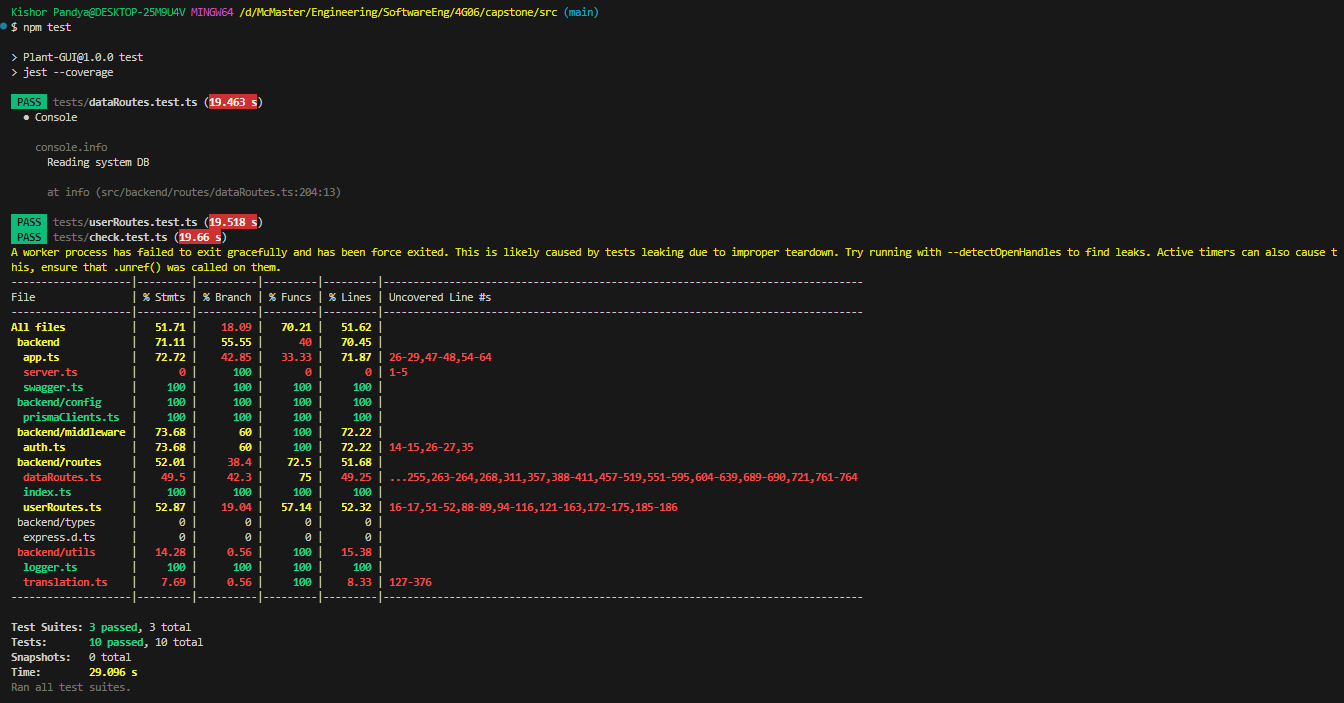
\includegraphics[width=\textwidth]{code_cov.png}
\end{figure}
If more you need more information on the code coverage, you need to run ``npm test'' and run the ``index.html'' file in the ``coverage'' folder which is autogenerated.

The reason the coverage is low is because we do not test all the endpoints since our frontend does not use all the endpoints opened by our backend. We have only tested the ones actively used by our frontend. Additionally, the frontend is tested using automated click-based testing which is not covered by the unit tests.
\bibliographystyle{plainnat}
\bibliography{../../refs/References}

\newpage{}
\section*{Appendix --- Reflection}

The information in this section will be used to evaluate the team members on the
graduate attribute of Reflection.

\input{../Reflection.tex}

\begin{enumerate}
  \item What went well while writing this deliverable? \\
   Kishor: Since our SRS document was well formatted and complete, it
   was easy to map the requirements to the tests.\\
   Dhrumil: The structure and format were clear from the start, which made it easy to keep everything consistent. Plus, the test cases were well-documented, so running and reporting them was straightforward. \\
   Madhu: Carrying out the manual tests with appropriate testers went well since our sponsor is heavily involved in the project. \\ 
   Rasik: Given the VNV plan a lot of the work creating the tables and test cases was done beforehand and quite reusable. This was very helpful to completing the work on a timely manner and it allowed us to focus on performing the tests\\
  \item What pain points did you experience during this deliverable, and how
    did you resolve them? \\
    Kishor: There were way too many non-functional requirements. It just got very boring after a bit.\\
    Dhrumil: Some tests needed adjustments to be practical for manual execution. To fix this, we introduced alternative monitoring methods, like tracking system resources and measuring response times. \\
    Madhu: Some of our tests felt repetitive since some of our requirements were closely related and therefore making tests for each requirement can become a little repetitive. \\
    Rasik: Working with outside testers was pain inducing, as they're not aware of the functionalities of the application. \\ 
  \item Which parts of this document stemmed from speaking to your client(s) or
  a proxy (e.g. your peers)? Which ones were not, and why?
  \\
  Our client wanted automated tests and so the unit testing/automated testing stemmed from our client. On the other hand we came up with the manual nfr and functional tests independantly since we found it important to have a set of manual tests to evaluate our ability to fulfill the system requirements. Similarly we came up with the changes based off of the test independantly since we were able to evaluate the causes of the failures in the test and use them to come up with appropriate changes/solutions. 
  \item In what ways was the Verification and Validation (VnV) Plan different
  from the activities that were actually conducted for VnV?  If there were
  differences, what changes required the modification in the plan?  Why did
  these changes occur?  Would you be able to anticipate these changes in future
  projects?  If there weren't any differences, how was your team able to clearly
  predict a feasible amount of effort and the right tasks needed to build the
  evidence that demonstrates the required quality?  (It is expected that most
  teams will have had to deviate from their original VnV Plan.) \\
  In our VnV plan we initially planned on having a larger suit of unit tests and automated tests as we expected to use our unit tests/automated tests to provide full coverage of our frontend codebase. However in practice we realized that our frontend was too complicated and the codebase was too large to effectively test it with full code coverage using just unit tests. This is why we eventually swapped to a more manual testing based approach in the VnV report and did not have as many unit tests. Instead we mainly just used unit tests for our backend systems and relied on manual testing for the frontend. In the future we can avoid this issue by setting appropriate expectations on the level of complexity of the codebase and be realistic about how many code based unit tests we can setup for a complex codebase. 
\end{enumerate}

\end{document}
